We formulate NLG as a planning problem on a Markov decision process
(MDP)~\cite{puterman_1994_markov}. An MDP is a tuple $(S, A, T, R, \gamma)$ where $S$ is a
set of states, $A$ is a set of actions available to an agent,
$T:S\times A\times S \rightarrow (0,1)$ is a possibly stochastic
function defining the probability $T(s,a,s')$ with which the
environment transitions to $s'$ when the agent does $a$ in state $s$.
$R:S\times A \rightarrow \mathbb{R}$ is a real-valued reward function that
specifies the utility of performing action $a$ in state $s$. Finally,
$\gamma$ is a discount factor that allows planning over infinite
horizons to converge. In such an MDP, the agent selects actions at
each state (a {\em policy}) to optimize the expected long-term
discounted reward: $\pi^*(s)=\arg \max_a E(\sum_t \gamma^t
R(s_t,a_t)|s=s_0)$, where the expectation is taken with respect to the
state transition distribution.

When the MDP model ($T$ and $R$) is
known, various dynamic programming algorithms such as value
iteration~\cite{bellman_1957_dynamic} can be used to plan and act in an MDP. When the
model is unknown, and the task is to formulate a policy, it can be
solved in a model-free way (i.e. without estimating $T$ and $R$)
through temporal difference (TD) learning. The key idea in TD-learning
is to take advantage of Monte Carlo sampling; since the agent visits
states and transitions with a frequency governed by the unknown
underlying $T$, simply keeping track of average rewards over time
yields the expected values required to compute the optimal actions at
each state.

Determining the optimal policy at {\em every} state using the above
strategy is polynomial in the size of the state-action
space~\cite{brafman_2003_rmax}, which is intractable in our case. But for our application, we do not
need to find the optimal policy. Rather we just need to {\em plan} in
an MDP to achieve a {\em given} communicative goal. Is it
possible to do this without exploring the entire state-action space?
Recent work answers this question affirmatively. New techniques such
as sparse sampling~\cite{kearns_1999_sparse} and
UCT~\cite{kocsis_bandit_2006} show how to generate near-optimal plans
in large MDPs with a time complexity that is independent of the state
space size. Using such an approach with a suitable defined MDP
(explained below) allows us to naturally handle
probabilistic grammars as well as formulate NLG as a planning problem,
unifying the distinct lines of attack described above. Further, the
strong theoretical guarantees of UCT translate into fast generation in
many cases, as we demonstrate in our experiments.
As the state space size in the language generation MDP is
very large, we use a variation of the UCT algorithm in our system,
described below. 


Online planning in MDPs generally follows two steps. From each state
encountered, a lookahead tree is constructed and used to estimate the
utility of each action in this state. Then, the best action is taken,
the system transitions to the next state and the procedure is
repeated. In order to build a lookahead tree, a ``rollout policy'' is
used. This policy has two components: if it encounters a state already
in the tree, it follows a ``tree policy,'' discussed further below. If
it encounters a new state, the policy reverts to a ``default'' policy
that typically randomly samples an action. In all cases, any rewards
received during the rollout search are backed up. Because this is a
Monte Carlo estimate, typically, several simultaneous trials are run,
and we keep track of the rewards received by each choice and
use this to select the best action at the root.

The final detail that UCT specifies is the method for determining the tree policy.
The tree policy needed by UCT for a state $s$ is the action $a$ in that state which maximizes:
\begin{equation}
P(s,a) = Q(s,a) + c\sqrt{\frac{ln N(s)}{N(s,a)}}\label{eqn:uct}
\end{equation}
Here $Q(s,a)$ is the estimated value of $a$ as observed in the tree
search and $N(s)$ and $N(s,a)$ are visit counts for the state and
state-action pair. Thus the second term is an exploration term that
biases the algorithm towards visiting actions that have not been
explored enough. $c$ is a constant that trades off exploration and
exploitation. This essentially treats each action decision
as a bandit problem; previous work shows that this approach can
efficiently select near-optimal actions at each state.

We now describe our approach, called Sentence Tree Realization with
UCT (STRUCT). The states of the underlying MDP contain {\em partial
  sentences} along with their parse trees. The actions available at a
state allow refinements to the partial sentences. In particular, the
algorithm may choose an available nonterminal in the current parse
tree for a substitution or adjoin operation from a (possibly
probabilistic) LTAG. Given a nonterminal choice and a fixed
probabilistic lexicalized TAG (PLTAG), a well defined probability
distribution is induced over possible next states (possibly uniform if
just an LTAG is used).   Since trees in LTAGs are associated
with individual words, they can be interpreted as adding a specific
semantic meaning to the overall sentence while describing precisely
the syntactic environment in which these words can occur, and can even
define any arguments for the word in question, for instance, the
location of the subject and object of a verb, or the presence of a
required third argument.  Further, since all recursive phenomena are
encoded in auxiliary trees, it factors recursion from the domain of
dependencies \cite{bauer2009statistical}, and can add auxiliary trees
to partial sentences without breaking dependency links between nodes.
In situations where the sentence is complete (no nonterminals without
children), we add a dummy action to stop generation and emit the
sentence.  Note that a complete sentence does not necessarily imply
a terminal state because adjoin operations can still be performed
(e.g. ``The dog ran'' could be expanded to ``The black dog ran quickly'').

In order to control the search space, we restrict the structure of the
MDP so that while substitutions are available, only those operations
are considered when determining the distribution over the next state,
without any adjoins.  We do this is in order to generate a
complete and valid sentence quickly.  This allows STRUCT to operate as
an anytime algorithm, described further below.

 The transition distribution in
 the underlying MDP is implicitly defined by the probabilities
 associated with a PLTAG, or uniform in the case of a standard LTAG.
\begin{figure}[t]
\centering
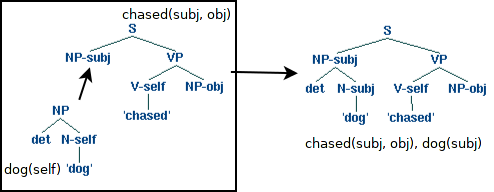
\includegraphics[width= 0.7 \linewidth]{sub-example.png}\label{examples}
\caption{An example tree substitution operation in STRUCT.}
\end{figure}

 In order to interact with the communicative goal, each word in our
 grammars consists of two components, a grammar entry and a lexicon
 entry.  A grammar entry has a name, a tree, and a set of annotations.
 These annotations contain data about how the syntactic data (the tree
 itself) interacts with the semantic data.  A lexicon entry has a word
 and a list of meanings.  These meanings are written as functions in
 first order logic, and can use as arguments the objects defined by
 the tree. This representation is similar to that used by
 CRISP~\cite{koller_sentence_2007}. In Figure~\ref{examples} we shown
 an example of a substitution operation applying an LTAG production to
 a chosen nonterminal in a partial sentence, and the associated
 semantic information.
 The grammar is made up of paired grammar entries and lexicon entries.
 See Figure \ref{examples} for example usage.

 While the production probabilities in the given PLTAG define the
 global structure of the state space, we use the reward function of
 the MDP to encode the specific communicative goal we are after. Since
 each state contains a partial sentence with its associated semantic
 information, we use this to evaluate the algorithm's progress towards
 the goal, and reward is allocated based on this progress. A key
 advantage of STRUCT over current techniques is our ability to specify
 a detailed reward function that captures complex communicative goals.
 For example, we can give ``progress'' rewards for partial sentences
 that achieve some parts of the communicative goal; we can penalize
 the algorithm if it attempts to generate a sentence that communicates
 something we wish {\em not} to communicate; we can trade off the
 importance of multiple communicative goals in the same sentence; we
 can even set up the reward function to prefer global criteria such as
 ``readability'', if we so choose. Of course, once any sentence is
 found that achieves the complete communicative goal, a large reward
 is given. Since the algorithm keeps track of the cumulative reward,
 such a sentence becomes a candidate solution. During the search,
 since we use finite depth lookahead and wish to propagate long range
 rewards to the root, we use a discount factor of 1.


 With the MDP definition above, we use UCT to find a solution sentence
 (Algorithm~\ref{uct-code}). We modify the standard algorithm in two
 ways. First, in the action selection step, we select the action that
 leads to the best $P(s,a)$ over all simulations rather than the best
 {\em average} $P(s,a)$. We do this because the original formulation
 of UCT is designed to work in adversarial situations, in such cases,
 selecting the absolute best may be risky if the opponent can respond
 with something that can also lead to a very bad result. In our case,
 however, there is no opponent, so we can freely choose the action
 leading to best overall reward. Second, after every action is
 selected and applied, we check to see if we are in a state in which
 the algorithm could terminate (i.e. the sentence has no nonterminals
 yet to be expanded).  If so, we determine if this is the best
 possibly-terminal state we have seen so far.  If so, we store it, and
 continue the generation process. If we reach a state from which we
 cannot continue generating, we begin again from the start state of
 the MDP. Because of the structure restriction above (substitution
 before adjoin), STRUCT also generates a valid sentence quickly. These
 modifications enable STRUCT to perform as an anytime algorithm, which
 if interrupted will return the highest-value complete and valid
 sentence.

After this point, any time that there are no substitutions
available (all nonterminals have at least one child), we record the
current sentence and its associated reward.  Such a sentence is
guaranteed to be both grammatical and complete.  If generation is
interrupted, we return the highest-value complete and valid sentence.
In this way, our approach functions as an anytime algorithm.

 We note that neither of these modifications cause any loss of
 generality.  Our Anytime-UCT implementation will work on any suitably
 defined MDP.  We implemented the system in Python 2.7. The pseudocode
  is shown in Algorithm~\ref{uct-code}.

 Clearly, the action set can get very large for a large grammar or for
 a long sentence with many locations for adjoining.  Still, this is the
 only way to ensure that we can generate all possible grammatical
 sentences.  UCT deals very well with this large action set due to the
 pruning inherent in its iterated Monte Carlo sampling method.  We can
 further compensate for this large action set by increasing the number
 of samples, if necessary.  It should also be noted that most
 combinations of these actions are order-independent; for instance, two
 actions, each adjoining an adjective to the subject and object of the
 sentence, respectively.  It is also notable that, occasionally, the
 order of some words in a sentence is not important.  ``A small white
 teapot'' and ``a white small teapot'' convey the same semantic
 information despite the different ordering of their adjectives.

\subsection{AI Planning}

Previously, those who interpret the sentence generation problem as planning have primarily used optimal planners to solve these planning problems.  CRISP is a prime example of this.  In other domains, there has been recent interest in probabilistic planners.  Monte Carlo Tree Search and, more specifically, the Upper Confidence bound applied to Trees (UCT), are exemplars of this subfield.\\

The UCT algorithm has already been shown to provide significant performance improvements for games played out using a minimax tree \cite{kocsis_bandit_2006}.  When compared with alpha-beta planning, Monte-Carlo planning, and Monte-Carlo planning with minimax value update, UCT was able to provide a lower failure rate with fewer iterations required.  It was shown that the number of iteration required for UCT to have an error rate of 0 converged to the same value as the alpha-beta algorithm.  However, if a smaller error rate was tolerated, the reduction in the number of iterations required could be significant.\\

The UCT algorithm can be used for natural language generation with some modifications.  Chevelu et al. \cite{chevelu_introduction_2009} used a variation of UCT, Monte Carlo Paraphrase Generation, in order to search through the possibilities afforded by a paraphrase table.  The principal modification, which we have adopted, is to select the action which leads to the best reward, instead of the best average reward.  This change is primarily motivated by the lack of adversary in the generation task, which was not the case in the game-playing initial conception of UCT.
\subsection{UCT}

\begin{algorithm}[t]
\caption{The STRUCT Algorithm.}\label{uct-code}
\begin{algorithmic}[1]
\REQUIRE Number of simulations $numTrials$, Depth of lookahead $maxDepth$
\ENSURE Generated sentence tree
\STATE $bestSentence \gets$ nil
\WHILE {User has not interrupted generation}
\STATE $state \gets$ empty sentence tree
\WHILE{$state$ not terminal}
	\FOR{$numTrials$}
		\STATE $testState \gets state$
		\STATE $currentDepth \gets 0$
		\IF{$testState$ has unexplored actions}
			\STATE Apply one unexplored PLTAG production chosen
                        uniformly at random to $testState$
			\STATE $currentDepth$++
		\ENDIF
		\WHILE{$currentDepth < maxDepth$}
			\STATE Apply PLTAG production selected by tree
                        policy (Equation~\ref{eqn:uct})
			\STATE $currentDepth$++
		\ENDWHILE
		\STATE calculate reward for $testState$
		\STATE associate reward with first action taken
	\ENDFOR
	\STATE $state \gets$ maximum reward $testState$
	\IF{$state$ score $> bestSentence$ score \AND $state$ has no nonterminal leaf nodes}
		\STATE $bestSentence \gets state$
	\ENDIF
\ENDWHILE
\ENDWHILE
\RETURN $bestSentence$
\end{algorithmic}
\caption{Pseudocode explanation of UCT}
\label{uct-code}
\end{algorithm}

UCT(Upper Confidence bound applied to Trees) \cite{kocsis_bandit_2006} is a planning algorithm that takes advantage of Monte-Carlo sampling to prune large sections of the search space each iteration.  Actions are sampled from each possible action at each state, and an action is chosen immediately based on the best average reward found.  This algorithm can handle large search-spaces since it prunes a large percentage of the search space with each action.  As it takes more samples per round, it increases the likelihood that it will prune only portions of the search space that do not contain the best output increases.\\

Our modifications of UCT in order to improve its use in the specific natural language generation task are show in Figure \ref{uct-code}.  Unlike in the game-playing task for which UCT was designed, we have no adversary in this generation task, and therefore we seek the best path that we have found so far, rather than the maximum average-value path.  We have found that UCT, modified in this way, provides excellent optimal and near-optimal outputs.  In addition, due to the way that we have structured our action definition, we use UCT as an anytime algorithm; we first generate the simplest and shortest valid sentence first, and increasingly improve the sentence over time until the sentence can no longer be improved.\\

Our choice of UCT is motivated by the high branching factor encountered in natural language generation when dealing with large grammars as well as the belief that optimal sentences to accomplish a communicative goal are not required in most discourse.  In fact, generating optimal sentences may be more time-consuming than nearly-optimal plans which accomplish the goal nearly as well.\\

In order to further improve the runtime of our approach, we introduced parallel processing into the UCT generation.  To do this, multiple processes are spawned, each running the generation steps and returning back the best action.  Then, the best actions found from each process will be compared and the action resulting in the best reward will be executed.  This allows for many more samples to be run in a system with multiple processors or capable of executing many threads at once, resulting in a better action being discovered in fixed time..\\

The process of generation can be split into four components:

\subsubsection{Tree Policy}
Starting from the current state, an action will repeatedly be chosen based on a balance of exploration and exploitation, until a state with an open action is hit, a leaf is hit, of the depth limit is reached.  The balance between exploration and exploitation is maintained by probabilistically selecting actions based on their expected value and the number of samples taken from that state.  More precisely:

$$P(a) = Q(s,a) + c\sqrt{\frac{ln n(s)}{n(s,a)}}$$

where $s$ is the current state, $a$ is the action from the current state, $c$ is an exploration constant, $n(s)$ is the number of times state $s$ has been encountered, $n(s,a)$ is the number of times action $a$ was taken in state s, P(a) is the probability that action $a$ is randomly selected, and $Q(s,a)$ is the expected value of state $s$ after selecting action $a$.

\subsubsection{State Expansion}
If there are any unexplored actions for the current state, choose one of the unexplored actions at random.  This will remove the chosen action from the open action list for that state.

\subsubsection{Default Policy}
Continue to select actions at random until either a terminal state or the depth limit is reached.

\subsubsection{Reward Assignment}
Calculate the reward function for the state that results after executing all of the chosen action and push the reward all the way back up to the root node representing the current state.

\subsection{STRUCT}

Here, we present STRUCT, 'Sentence Tree Realization using UCT', a statistical general-purpose natural language generator.  STRUCT is our implementation of the algorithm shown in Figure \ref{uct-code}, written in Python 2.

\subsubsection{Grammar Choice}

STRUCT supports Context Free Grammars (CFGs), Probabilistic Context Free Grammars (PCFGs), Tree Adjoining Grammars (TAGs), and Probabilistic Tree Adjoining Grammars (PTAGs).  For the experiments below, we primarily focus on a restricted subset of TAGs and PTAGs, the Lexicalized Tree Adjoining Grammars (LTAGs, PLTAGs).  LTAGs are TAGs in which each tree contains at least one word which will be present in the final sentence, an 'anchor word'.  CRISP, mentioned above, also uses LTAGs, which makes comparison between the generators simpler.\\

 LTAGs were chosen due to their interesting linguistic properties.  Since trees are associated with individual words, they can be interpreted as adding a specific semantic meaning to the overall sentence while describing precisely the syntactic environment in which these words can occur, and can even define any arguments for the word in question, for instance, the location of the subject and object of a verb, or the presence of a required third argument.  Further, since all recursive phenomena are encoded in auxiliary trees, we have removed recursion from the domain of dependencies \cite{bauer2009statistical}, and can add auxiliary trees to our partial sentences without breaking dependency links between nodes.

 \subsubsection{Action Definition}

 Actions in STRUCT are applications of a particular grammar rule to a specific node in the partial tree.  In a context-free grammar and in the case of an initial tree in a TAG, these are determined by iterating through all leaf nonterminals and adding a possible action for each rule in the grammar applicable at this point.  Adjoining trees in a TAG are determined by iterating through each node in the tree and adding a possible action for each adjoining tree applicable at that point.\\


 \subsubsection{Reward Function Definition}

 The reward function for a state must be defined exclusively in terms
 of the state in question.  The reward function serves as a metric to
 rank the favorableness of a sentence.  This reward function must be
 efficiently computable since it will be computed for every iteration
 in the UCT algorithm.  It must also be able to provide a value for a
 partial sentence since, due to the depth limit, a complete sentence
 may not always be reached.

% \begin{figure}
% \begin{algorithmic}
% \Function{reward}{$tree$, $terminal$, $semantic\_goal$}
% \State $reward \gets$ 0
% 	\For{each $subtree$ in $tree$}
% 		\If{$subtree$ satisfies $semantic\_goal$}
% 		\State $reward \gets reward + 1000$
% 			\For{each $semantic\_argument$ of $subtree$}
% 			\State $refs \gets$ all possible referents
% 			\If {intended reference in $refs$}
% 			\State $reward \gets reward + 300 / len(refs)$
% 			\EndIf
% 			\EndFor
% 		\State \bf{break}
%		\EndIf
%	\EndFor
%\If{$terminal$}
%$reward \gets reward + .00001$
%\EndIf
%\State \Return reward
%\EndFunction
%\end{algorithmic}
%\label{alg-crisp-emulator}
%\caption{Reward Function used to emulate CRISP}
%\end{figure}
